% -*- latex -*-
%%%%%%%%%%%%%%%%%%%%%%%%%%%%%%%%%%%%%%%%%%%%%%%%%%%%%%%%%%%%%%%%
%%%%%%%%%%%%%%%%%%%%%%%%%%%%%%%%%%%%%%%%%%%%%%%%%%%%%%%%%%%%%%%%
%%%%
%%%% This text file is part of the source of 
%%%% `Parallel Programming in MPI and OpenMP'
%%%% by Victor Eijkhout, copyright 2012-2021
%%%%
%%%% mpi-persist.tex : persistent communication and such
%%%%
%%%%%%%%%%%%%%%%%%%%%%%%%%%%%%%%%%%%%%%%%%%%%%%%%%%%%%%%%%%%%%%%
%%%%%%%%%%%%%%%%%%%%%%%%%%%%%%%%%%%%%%%%%%%%%%%%%%%%%%%%%%%%%%%%

\Level 0 {Persistent communication requests}
\index{persistent communication|see{communication, persistent}}
\label{sec:persistent}

Persistent communication is a mechanism for dealing
with a repeating communication transaction,
where the parameters of the transaction,
such as sender, receiver, tag, root, and buffer type and size,
stay the same.
Only the contents of the buffers involved changes between the transactions.

You can imagine that setting up a communication
carries some overhead, and if the same communication structure
is repeated many times, this overhead may be avoided.

\begin{enumerate}
\item
  For nonblocking communications \lstinline{MPI_Ixxx}
  (both point-to-point and collective)
  there is a persistent variant \n{MPI_Xxx_init}
  with the same calling sequence.
  The `init' call produces
  an \indexmpishow{MPI_Request} output parameter,
  which can be used to test for completion of the communication.
\item 
  The `init' routine does not start the actual communication:
  that is done in
  \indexmpidef{MPI_Start},
  or \indexmpidef{MPI_Startall} for multiple requests.
\item Any of the MPI `wait' calls can then be used
  to conclude the communication.
\item The communication can then be restarted with another `start' call.
\item The wait call does not release the request object,
  since it can be used for repeat occurrences of this transaction.
  The request object is freed, as usual, with \indexmpishow{MPI_Request_free}.
\end{enumerate}

\begin{lstlisting}
MPI_Send_init( /* ... */ &request);
while ( /* ... */ ) {
  MPI_Start( request );
  MPI_Wait( request, &status );
}
MPI_Request_free( & request );
\end{lstlisting}

\begin{mplnote}{Persistent requests}
  MPL returns a \indexmpldef{prequest}
  from persistent `init' routines, rather than an \indexmplshow{irequest}
  (MPL note~\ref{mpl:irequest}):
\begin{lstlisting}
template<typename T >
prequest send_init (const T &data, int dest, tag t=tag(0)) const;
\end{lstlisting}
Likewise, there is a \indexmpldef{prequest_pool}
instead of an \indexmplshow{irequest_pool} (note~\ref{mpl:req_pool}).
\end{mplnote}

\Level 1 {Persistent point-to-point communication}
\label{sec:persist-p2p}
\index{persistent!point-to-point|(textbf}

The main persistent point-to-point routines are
\indexmpishow{MPI_Send_init}, which has the same calling sequence as
\indexmpishow{MPI_Isend}, and \indexmpishow{MPI_Recv_init}, which has the same
calling sequence as \indexmpishow{MPI_Irecv}.
  
In the following example a ping-pong is implemented with persistent communication.
Since we use persistent operations for both send and receive on the `ping' process,
we use \indexmpishow{MPI_Startall} to start both at the same time,
and \indexmpishow{MPI_Waitall} to test their completion.
%  
\cverbatimsnippet[examples/mpi/c/persist.c]{persist}
%
\pverbatimsnippet[examples/mpi/p/persist.py]{persistp}

As with ordinary send commands, there are persistent variants
\begin{itemize}
\item
  \indexmpishow{MPI_Bsend_init} for buffered communication,
  section~\ref{sec:buffered};
\item
  \indexmpishow{MPI_Ssend_init} for synchronous communication,
  section~\ref{sec:syncsend};
\item
  \indexmpishow{MPI_Rsend_init}.
\end{itemize}

\index{persistent!point-to-point|)}

\Level 1 {Persistent collectives}

\begin{mpifour}
% https://github.com/mpi-forum/mpi-issues/issues/25
\index{persistent!collectives|(textbf}
For each collective call, there is a persistent variant (\mpistandard{4}).
As with persistent point-to-point calls (section~\ref{sec:persist-p2p}),
these have the same calling sequence as the nonpersistent variants,
except for an added final \indexmpishow{MPI_Request} parameter.
This request (or an array of requests) can then be used by
\indexmpishow{MPI_Start} (or \indexmpishow{MPI_Startall})
to initiate the actual communication.

Some points.
\begin{itemize}
\item
  Metadata arrays, such as of counts and datatypes,
  must not be altered until the \indexmpishow{MPI_Request_free} call.
\item The initialization call is nonlocal, so it can block until all
  processes have performed it.
\item Multiple persistent collective can be initialized, in which case
  they satisfy the same restrictions as ordinary collectives, in particular
  on ordering. Thus, the following code is incorrect:
\begin{lstlisting}
// WRONG
if (procid==0) {
  MPI_Reduce_init( /* ... */ &req1);
  MPI_Bcast_init( /* ... */ &req2);
} else {
  MPI_Bcast_init( /* ... */ &req2);
  MPI_Reduce_init( /* ... */ &req1);
}
\end{lstlisting}
However, after initialization the start calls can be in arbitrary order,
and in different order among the processes.
\end{itemize}

\begin{raggedlist} %pyskip
  Available persistent collectives are:
  \indexmpidef{MPI_Barrier_init}
  \indexmpidef{MPI_Bcast_init}
  \indexmpidef{MPI_Reduce_init}
  \indexmpidef{MPI_Allreduce_init}
  \indexmpidef{MPI_Reduce_scatter_init}
  \indexmpidef{MPI_Reduce_scatter_block_init}
  \indexmpidef{MPI_Gather_init}
  \indexmpidef{MPI_Gatherv_init}
  \indexmpidef{MPI_Allgather_init}
  \indexmpidef{MPI_Allgatherv_init}
  \indexmpidef{MPI_Scatter_init}
  \indexmpidef{MPI_Scatterv_init}
  \indexmpidef{MPI_Alltoall_init}
  \indexmpidef{MPI_Alltoallv_init}
  \indexmpidef{MPI_Alltoallw_init}
  \indexmpidef{MPI_Scan_init}
  \indexmpidef{MPI_Exscan_init}
\end{raggedlist} %pyskip

\index{persistent!collectives|)}
\end{mpifour}

\Level 1 {Persistent neighbor communications}

\begin{mpifour}

  \begin{raggedlist} %pyskip
    \indexmpidef{MPI_Neighbor_allgather_init},
    \indexmpidef{MPI_Neighbor_allgatherv_init},
    \indexmpidef{MPI_Neighbor_alltoall_init},
    \indexmpidef{MPI_Neighbor_alltoallv_init},
    \indexmpidef{MPI_Neighbor_alltoallw_init},
  \end{raggedlist} %pyskip

\end{mpifour}

\Level 0 {Partitioned communication}
\begin{mpifour}
\label{sec:psend}
\index{partitioned communication|(}
\index{communication!partitioned|see{partitioned,communication}}

Partitioned communication is a variant
on \indextermbus{persistent}{communication},
where a message is constructed in partitions.
\begin{itemize}
\item The normal \indexmpishow{MPI_Send_init} is replaced
  by \indexmpidef{MPI_Psend_init}.
\item After this, the \indexmpishow{MPI_Start} does not
  actually start the transfer; instead:
\item Each partition of the message is separately
  declared as read-to-be-sent with \indexmpishow{MPI_Pready}.
\end{itemize}
A common scenario for this is in multi-threaded environments,
where each thread can construct its own part of a message.
Having partitioned messages means that partially constructed message buffers
can be sent off without having to wait for all threads to finish.

Indicating that parts of a message are ready for sending
is done by one of the following calls:
\begin{itemize}
\item \indexmpidef{MPI_Pready} for a single partition;
\item \indexmpidef{MPI_Pready_range} for a range of partitions; and
\item \indexmpidef{MPI_Pready_list} for an explicitly enumerated list of partitions.
\end{itemize}
The \indexmpishow{MPI_Psend_init} call yields an \indexmpishow{MPI_Request} object
that can be used to test for completion
(see sections \ref{sec:waittest} and~\ref{sec:mpitest})
of the full operation started with
\indexmpishow{MPI_Start}.

On the receiving side:
\begin{itemize}
\item A call to \indexmpishow{MPI_Recv_init} is replaced by
  \indexmpidef{MPI_Precv_init}.
\item Arrival of a partition can be tested with \indexmpidef{MPI_Parrived}.  
\end{itemize}
Again, the \indexmpishow{MPI_Request} object from the receive-init call can
be used to test for completion of the full receive operation.

\index{partitioned communication|)}
\end{mpifour}

\Level 0 {Synchronous and asynchronous communication}
\index{communication!synchronous|(textbf}
\index{communication!asynchronous|(textbf}

It is easiest to think of blocking as a form of synchronization with
the other process, but that is not quite true. Synchronization is a
concept in itself, and we talk about \emph{synchronous} communication
if there is actual coordination going on with the other process,
and \emph{asynchronous} communication if there is not. Blocking then
only refers to the program waiting until the user data is safe
to reuse; in the synchronous case a blocking call means that the data
is indeed transferred, in the asynchronous case it only means that the
data has been transferred to some system buffer.
%
\begin{figure}[ht]
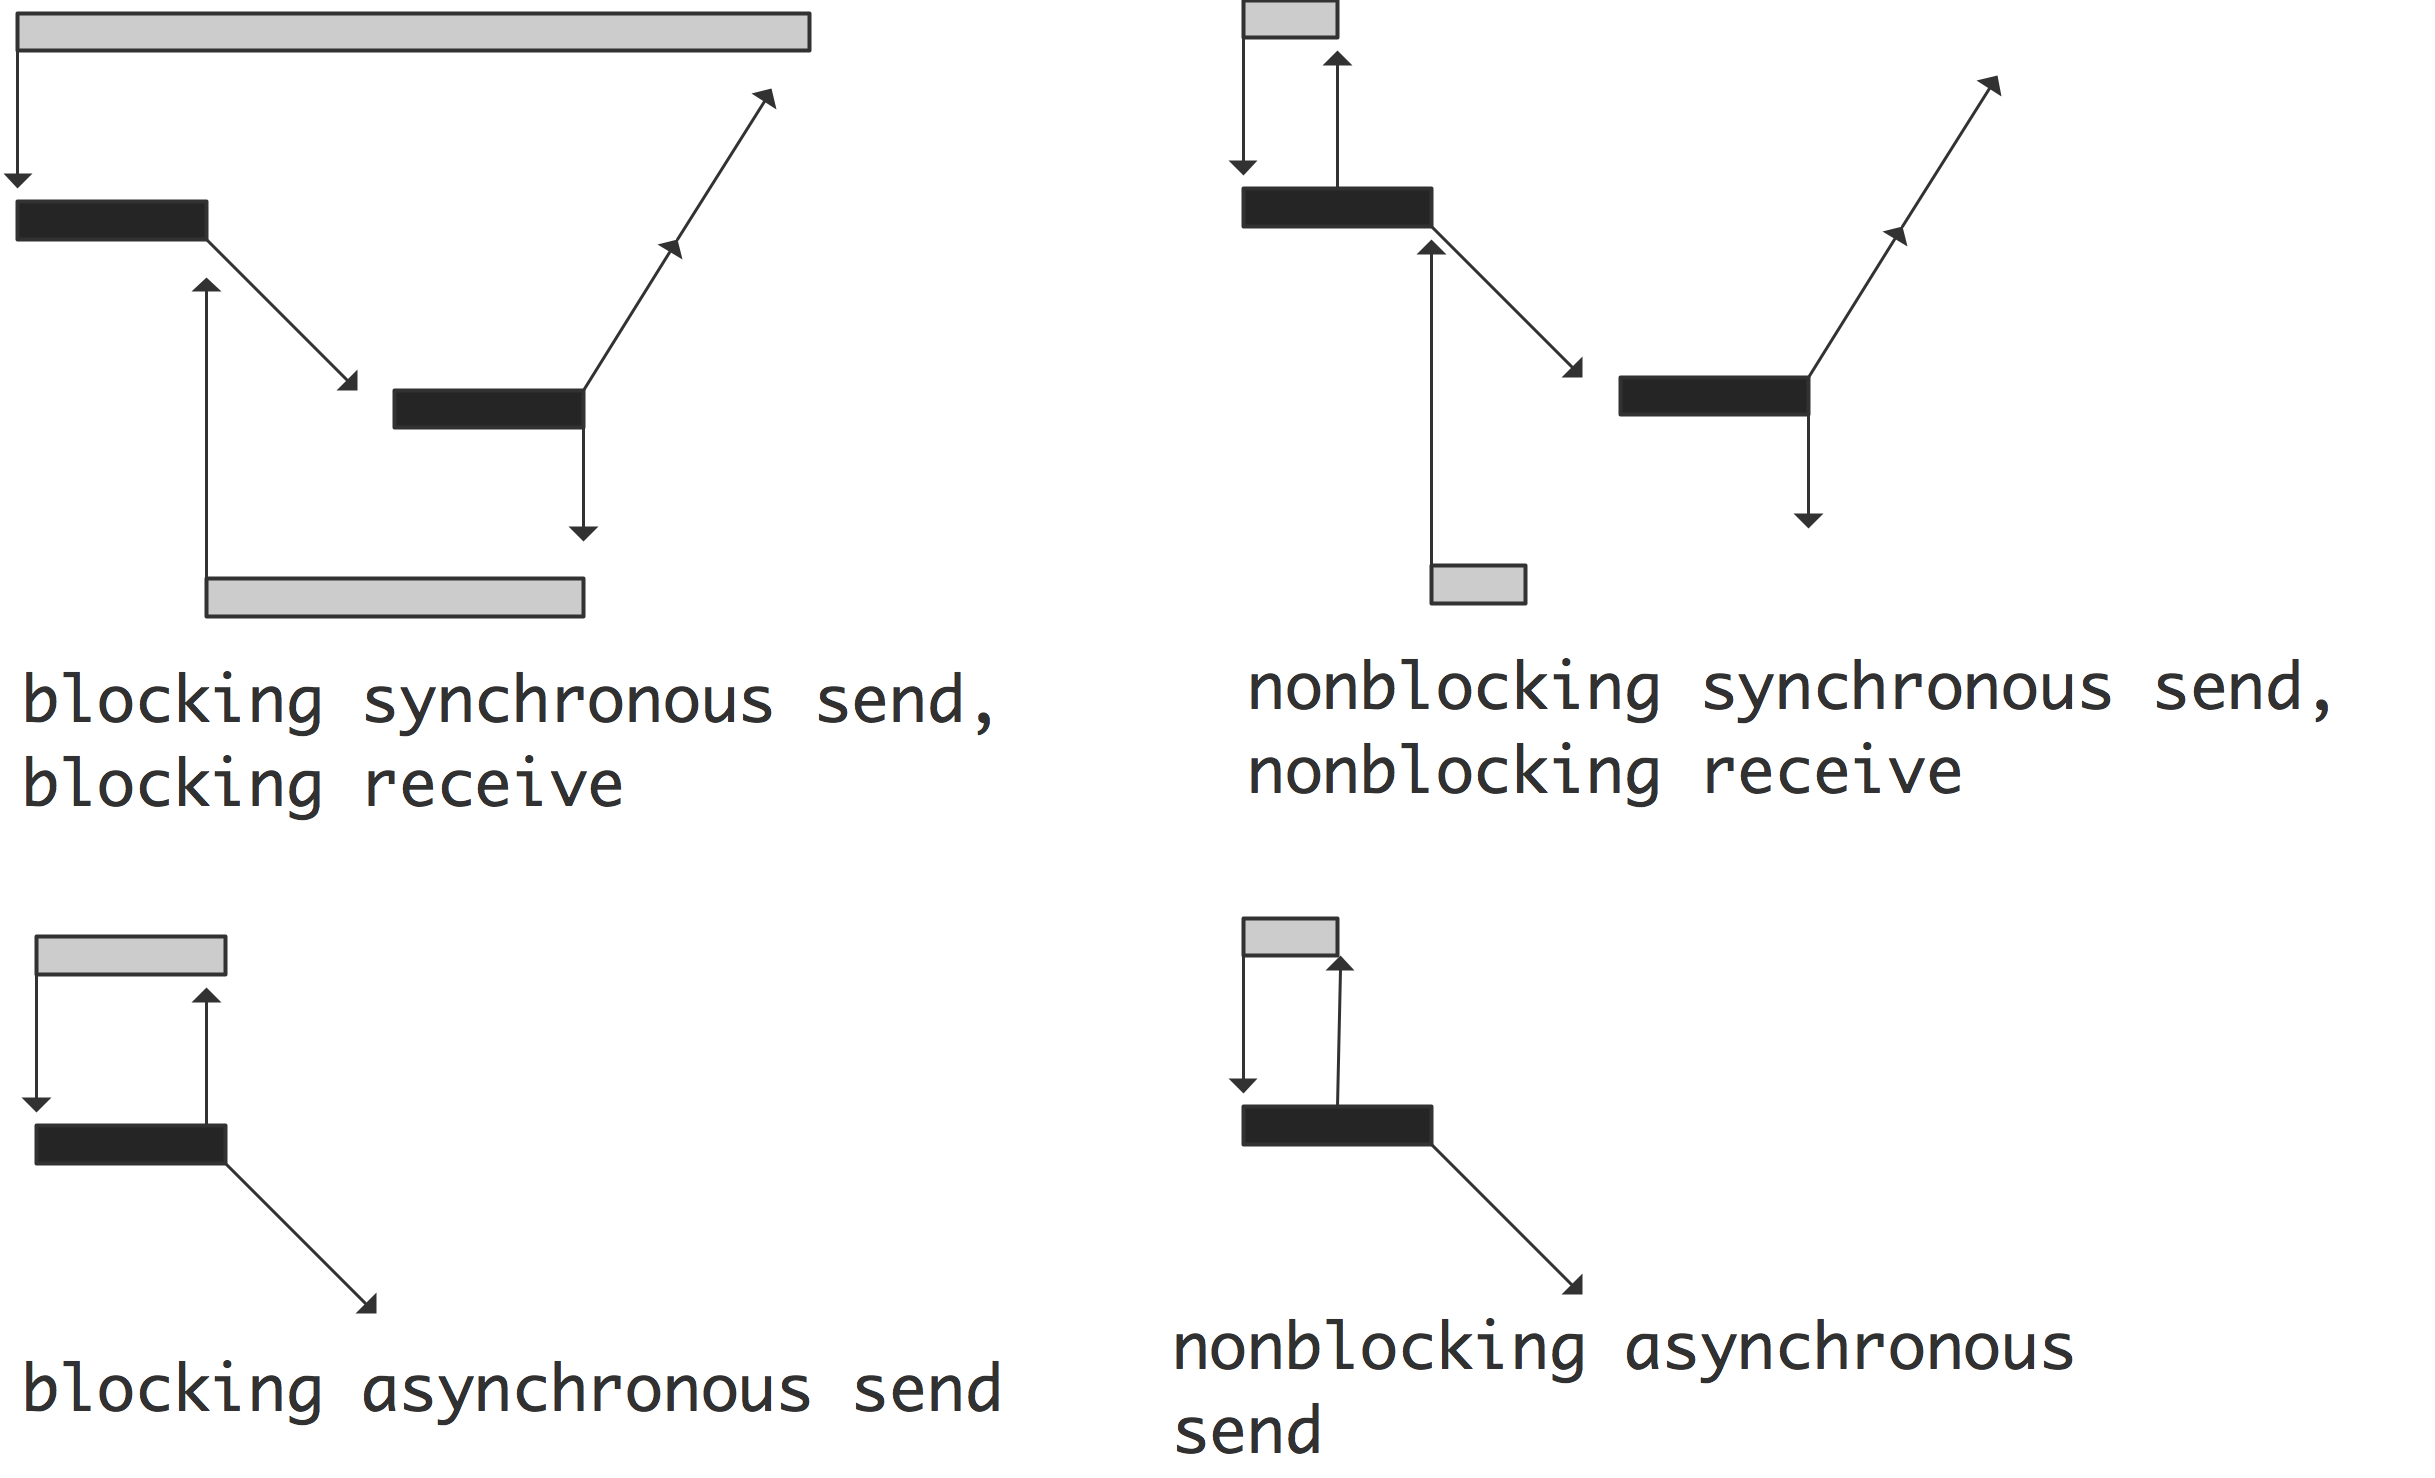
\includegraphics[scale=.15]{block-vs-sync}
\caption{Blocking and synchronicity}
\label{fig:block-sync}
\end{figure}
The four possible cases are illustrated in figure~\ref{fig:block-sync}.

\Level 1 {Synchronous send operations}
\label{sec:syncsend}

MPI has a number of routines for synchronous communication,
such as \indexmpidef{MPI_Ssend}.
Driving home the point that nonblocking and asynchronous are
different concepts, there is a routine \indexmpidef{MPI_Issend},
which is synchronous but nonblocking.
These routines have the same calling sequence as their not-explicitly
synchronous variants, and only differ in their semantics.

See section~\ref{sec:eager-limit} for examples.

\index{communication!synchronous|)}
\index{communication!asynchronous|)}

\Level 0 {Local and nonlocal operations}
\label{sec:mpi-local-non}
\label{sec:local-non-send}
\index{communication!local|(textbf}
\index{communication!nonlocal|(textbf}

The MPI standard does not dictate whether communication is buffered.
If a message is buffered, a send call can complete,
even if no corresponding send has been posted yet.
See section~\ref{sec:eager-limit}.
Thus, in the standard communication, a send operation
is \emph{nonlocal}: its completion may be depend on
whether the corresponding receive has been posted.
A \indextermbusdef{local}{operation} is one that is not nonlocal.

On the other hand, \indextermsub{buffered}{communication}
(routines \indexmpishow{MPI_Bsend}, \indexmpishow{MPI_Ibsend},
\indexmpishow{MPI_Bsend_init}; section~\ref{sec:buffered})
is \emph{local}:
the presence of an explicit buffer means that a send operation
can complete no matter whether the receive has been posted.

The \indextermsub{synchronous}{send} 
(routines \indexmpishow{MPI_Ssend}, \indexmpishow{MPI_Issend},
\indexmpishow{MPI_Ssend_init}; section~\ref{sec:handshake})
is again nonlocal (even in the nonblocking variant)
since it will only complete when the receive call has completed.

Finally, the \indextermsub{ready mode}{send}
(\indexmpishow{MPI_Rsend}, \indexmpishow{MPI_Irsend})
is nonlocal in the sense that its only correct use
is when the corresponding receive has been issued.

\index{communication!local|)}
\index{communication!nonlocal|)}

\Level 0 {Buffered communication}
\label{sec:buffered}

\begin{figure}[ht]
  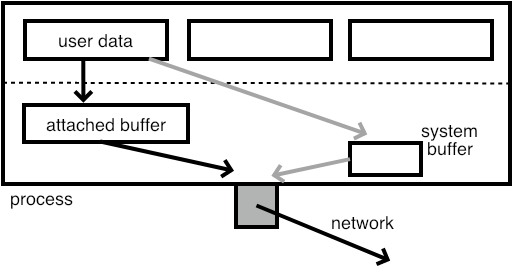
\includegraphics[scale=.5]{bufferattach}
  \caption{User communication routed through an attached buffer}
  \label{fig:bufattach}
\end{figure}

By now you have probably got the notion that managing buffer
space in MPI is important: data has to be somewhere, either in
user-allocated arrays or in system buffers. Using
\indextermsubdef{buffered}{communication} is yet another
way of managing buffer space.
\begin{enumerate}
\item You allocate your own buffer space, and you attach it to your
  process. This buffer is not a send buffer: it is a replacement for
  buffer space used inside the MPI library or on the network card;
  figure~\ref{fig:bufattach}. If high-bandwdith memory is available,
  you could create your buffer there.
\item You use the \indexmpiref{MPI_Bsend}
  (or its \emph{local}\index{local!operation} variant \indexmpishow{MPI_Ibsend})
  call for sending, using
  otherwise normal send and receive buffers;
\item You detach the buffer when you're done with the buffered sends.
\end{enumerate}

One advantage of buffered sends is that they are nonblocking:
since there is a guaranteed buffer long enough to contain the
message, it is not necessary to wait for the receiving process.

We illustrate the use of buffered sends:

\cverbatimsnippet{bsendbuf}

\Level 1 {Buffer treatment}

There can be only one buffer per process, attached with
\indexmpiref{MPI_Buffer_attach}.
Its size should be enough
for all \indexmpishow{MPI_Bsend} calls that are simultaneously
outstanding.
You can compute the needed size of the buffer with \indexmpishow{MPI_Pack_size};
see section~\ref{sec:pack}.
Additionally, a term of \indexmpidef{MPI_BSEND_OVERHEAD} is needed.
See the above code fragment.

The buffer is detached with \indexmpidef{MPI_Buffer_detach}:
\begin{lstlisting}
int MPI_Buffer_detach(
  void *buffer, int *size);
\end{lstlisting}
This returns the address and size of the buffer; the call blocks
until all buffered messages have been delivered.

Note that both
\indexmpishow{MPI_Buffer_attach} and \indexmpishow{MPI_Buffer_detach}
have a \lstinline+void*+ argument for the buffer, but 
\begin{itemize}
\item in the attach routine this is the address of the buffer,
\item while the detach routine it is the address of the buffer pointer.
\end{itemize}
This is done so that the detach routine can zero the buffer pointer.

While the buffered send is nonblocking like an \indexmpishow{MPI_Isend},
there is no corresponding wait call.
You can force delivery by
\begin{lstlisting}
MPI_Buffer_detach( &b, &n );
MPI_Buffer_attach( b, n );
\end{lstlisting}

\begin{mplnote}{Buffered send}
  Creating and attaching a buffer is done through \indexmpldef{bsend_buffer}
  and a support routine \indexmpldef{bsend_size} helps in calculating
  the buffer size:
  \cxxverbatimsnippet{bsendbufmpl}

  Constant: \lstinline+mpl::+\indexmplshow{bsend_overhead} is \lstinline{constexpr}'d
  to the MPI constant \indexmpishow{MPI_BSEND_OVERHEAD}.
\end{mplnote}

\begin{mplnote}{Buffer attach and detach}
  There is a separate attach routine, but normally this is called
  by the constructor of the \lstinline+bsend_buffer+.
  Likewise, the detach routine is called in the buffer destructor.
\begin{lstlisting}
void mpl::environment::buffer_attach (void *buff, int size);
std::pair< void *, int > mpl::environment::buffer_detach ();
\end{lstlisting}
\end{mplnote}

\Level 1 {Bufferend send calls}

The possible error codes are
\begin{itemize}
\item \indexmpishow{MPI_SUCCESS} the routine completed successfully.
\item \indexmpishow{MPI_ERR_BUFFER} The buffer pointer is invalid;
  this typically means that you have supplied a null pointer.
\item \indexmpishow{MPI_ERR_INTERN} An internal error in MPI has been detected.
\end{itemize}

The asynchronous version is \indexmpishow{MPI_Ibsend}, the persistent
(see section~\ref{sec:persistent}) call is \indexmpishow{MPI_Bsend_init}.

\Level 1 {Persistent buffered communication}

There is a persistent variant 
\indexmpiref{MPI_Bsend_init}
of buffered sends, as with regular
sends (section~\ref{sec:persistent}).

